\documentclass[UTF8]{article}
\usepackage{ctex}
\usepackage{ulem}
\usepackage{amssymb}
\usepackage{amsmath}
\usepackage{graphicx}
\newtheorem{thm}{定义}[section]
\newtheorem{notation}[thm]{记号}
\newtheorem{lemma}[thm]{引理}

\makeatletter
\newcommand{\rmnum}[1]{\romannumeral #1}
\newcommand{\Rmnum}[1]{\expandafter\@slowromancap\romannumeral #1@}
\makeatother
\newcommand{\dperp}{\perp\!\!\!\perp}

\title{10 $\lambda{\rm D}$的规则与性质\\Rules and properties of $\lambda{\rm D}$\\[2ex]\begin{large}读书笔记\end{large}}
\author{许博}
\date{}

\begin{document}
\maketitle
	\section{疑问}
	
		1. Axiom 和 Axiomatic notion 的区别是什么?

	\section{描述性定义与基本(primitive)定义}
	\noindent
	上一章中,我们定义了基于描述性定义的系统$\lambda{\rm D_0}$,将定义作为“一等公民”扩展了$\lambda{\rm C}$。其中“描述性”指的是每一个被定义的常量都与一个确切的定义实体(definien)相关联,并且被给定一个形式化的描述以表示这个常量代表了什么。
	
		而在通常的数学和逻辑中,还需要表示所谓的基本概念(primitive  notion),用于结合公理和公理性概念。
		
		基本定义中所引入的常量与描述性定义中相异的是,它不与一个描述性的表达式相关联,只提供它的类型,而没有更多的限制。因此,基本的常量也不能展开。
		
		一个基本定义可以被看作是公理性的引入逻辑或者数学中一个假设存在但不能构造出来的对象。同样可以在$\lambda{\rm C}$用于假设成立但无法证明的一个公理,比如在章节7.4中提到的DN公理。
		
		描述性定义和基本定义的本质区别在于定义实体(definien)的存在与否,而它们一致的地方在于:两者中常量的行为相似,都是它们参数列表的实例化;以及两者中的常量都关联于一个类型。
		
		因为这些相似性,我们选择将这两者的引入过程合二为一。也意味着我们将扩展“定义”到基本或者公理性的名字。
		
		以基本定义扩展$\lambda{\rm D_0}$后,得到的系统称为$\lambda{\rm D}$。系统$\lambda{\rm D}$是我们最终的形式化机器,非常适合形式化大量的数学,其中一个好处是,形式化的过程强制形式化的内容得到完全的验证。
		
	\section{公理和公理性概念(axiomatic notion)}
	\noindent
	公理(axiom)或者说基本实体(primitive  entity),是假定存在或成立的概念或原理(principle),它们是某一个理论的基础(fundamental),非常基本所以不能由其它实体构造或者推导。
	
		一些基本实体:\\
		- 自然数的集合$\mathbb{N}$,作为皮亚诺算术(Peano arithmetic)的一个基础;\\
		- $\mathbb{N}$中的数 0 以及后继函数 $s:\mathbb{N}\rightarrow\mathbb{N}$,作为$\mathbb{N}$的基础;\\
		- 皮亚诺算术中归纳法公理;\\
		- 策梅洛-弗兰克尔集合论中的公理;比如空集公理(存在一个没有元素的集合)。
		
		这些实体在对应的理论中都是基本的,并且它们可以是集合,集合中的元素或者命题的断言,因为作为基本的公理,所以不需要证明(归纳法,空集合)。
		
		在章节7.4中,我们建议将ET公理作为假设添加在上下文之前,一种前上下文(pre-context)。但是,这个解决方案无疑有一些缺陷:\\
		- 在复杂化更复杂的情况下的推导,尤其是必须包含一些基本实体时,需要引入相当大的前上下文,比如需要自然数集合时,就需要先引入$\mathbb{N}$以及0和$s$的声明;\\
		- 目前尚不清楚如何处理在一个上下文中出现的基本实体(这里我感觉尽管一个上下文中出现的基本实体在前上下文中声明,但是一个上下文并不存在它的声明,所以尚不清楚)。例如,我们可以在一个上下文(而不是在$P$上的全称量词)表示归纳法,如下:
		
		“令$P$是任意在$\mathbb{N}$上的谓词,公理地假设归纳法适用于$P$”,可以更形式化地表示为:
		
		归纳性质:在上下文$P:\mathbb{N}\rightarrow*_p$中,假设
		
		$P0\Rightarrow(\forall_{n\in\mathbb{N}}(Pn\Rightarrow P(sn))\Rightarrow\forall_{n\in\mathbb{N}}(Pn))$。
	
		因此我们选择另一种方式表示基本实体,不看作是整体的假设,而看作是不包含定义实体(definien)的定义。而这些情况记为基本实体的定义或者基本定义。
		
		使用符号$\dperp$表示在一个基本定义中不存在的定义实体(definien),以使用和描述性定义相同的形式。
		
		\begin{thm}(基本定义,定义,环境)\\
			(1) 一个基本定义具有形式$\overline{x}:\overline{A}\triangleright a(\overline{x}):=\dperp:N$;\\
			(2) 一个定义是描述性的或基本的;\\
			(3) 作为结果,一个环境,也即定义的列表,现在也包括基本定义。
		\end{thm}
	
		样例:\\
		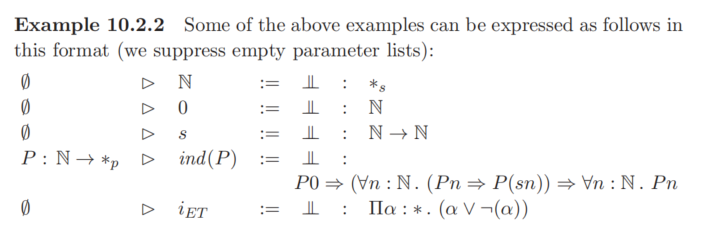
\includegraphics[width=0.93\linewidth]{"../imgs/10-1.png"}
		
		可以使用$ind(P)$用于在$\mathbb{N}$上的任意谓词$P$,通过应用推到规则($inst$)。
		
	\section{用于基本定义的规则}
	\noindent
	提供用于基本定义的推导规则。首先给出用于在环境中包含一个基本定义的规则。这个规则是($def$)的一个修改版本。
	
		因为基本定义中不存在定义实体,因此($def$)规则的第二个$\bf premiss$中的$M:N$修改为了$N:s$,以确保$N$是良构的:
		
		($def-prim$) 如果$a\notin\Delta$,则$\cfrac{\Delta;\Gamma\vdash K:L\ \ \ \Delta;\overline{x}:\overline{A}\vdash N:s}  {\Delta,\overline{x}:\overline{A}\triangleright a(\overline{x}):=\dperp:N;\Gamma\vdash K:L}$
		
		而对于实例化规则,唯一的修改在于定义中的$\dperp$:
		
		($inst-prim$) 如果$\overline{x}:\overline{A}\triangleright a(\overline{x}):=\dperp:N\in\Delta$,则$\cfrac{\Delta;\Gamma\vdash*:\square\ \ \ \Delta;\Gamma\vdash\overline{U}:\overline{A\left[\overline{x}:=\overline{U}\right]}}   {\Delta;\Gamma\vdash a(\overline{U}):N\left[\overline{x}:=\overline{U}\right]}$
		
		其中第一个$\bf premiss$,同样是为了保证在参数列表为空时,确保$\Delta;\Gamma$的良构。
		
		因为用于基本定义的规则($def-prim$)和($inst-prim$)与用于描述性定义的规则($def$)和($inst$)相似,因此值得并列,下图中框出了相关的语句,包括了两者中的相异之处:\\
		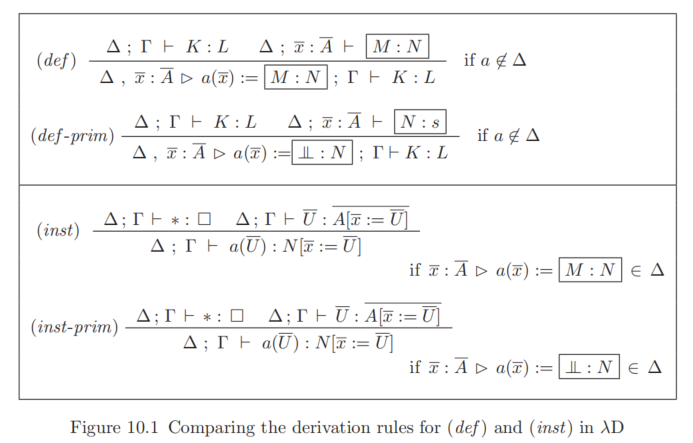
\includegraphics[width=0.93\linewidth]{"../imgs/10-2.png"}
		
		以规则($def-prim$)和($inst-prim$)扩展系统$\lambda{\rm D_0}$得到的系统记为$\lambda{\rm D}$。
		
	\section{$\lambda{\rm D}$的性质}
	\noindent
	$\lambda{\rm D}$中的大多数性质都是在$\lambda{\rm C}$中对应的性质上添加了定义的扩展,不再赘述。
	
	\section{$\lambda{\rm D}$中的规范化(normalisation)和汇流(confluence)}
	\noindent
	“规范化”是“终止”的另一个表示,因此我们观察规约关系$\rightarrow_\beta$和$\stackrel{\Delta}{\rightarrow}$的终止行为,包含各自以及组合的。终止被期望为是一个性质,因为它避免了无限的规约路径。回忆“弱规范化”和“强规范化”,前者存在一条到规范形式的路径,后者是所有的规约路径在若干步后都可以终止。而在$\lambda{\rm D}$中,在合法的环境和上下文中,关系$\rightarrow_\beta$和$\stackrel{\Delta}{\rightarrow}$的单独以及组合都满足“弱规范化”和“强规范化”。并且$\beta{\delta}$-规范形式是唯一的。
	
		对于汇流定理,关系$\rightarrow_\beta$和$\stackrel{\Delta}{\rightarrow}$的单独以及组合同样满足。不再赘述。
\end{document}
